% ============================================================
% Section 3: Proposed Method  (structure follows the Lymph reference paper)
% 3.1 = Fig.1(A)  3.2 = Fig.1(B)  3.3 = Fig.1(C)
% Preamble: \usepackage{graphicx,amsmath,amssymb,xcolor,soul}
% \tbd{...} = to be filled (yellow)
% ============================================================


\section{Proposed Method}

This work presents a calibration-free pipeline for estimating root canal filling
length from preoperative periapical radiographs. As illustrated in
Figure~\ref{fig:workflow}, the pipeline consists of three stages:
(A) dataset preparation, in which a YOLO11n detector extracts single-tooth images
from full periapical radiographs and the segmentation and length-evaluation
datasets are constructed; (B) tooth instance segmentation, in which each image is
enhanced by a morphological top-hat operation, spatially standardised, and
segmented by YOLO11n-seg; and (C) filling-length estimation, in which the pixel
length measured along the mask's longitudinal axis is normalised by the
radiograph's long side and converted to millimetres by Gaussian process
regression (GPR) with patient age, followed by a fixed safety offset. Each image
is processed independently, and the preprocessing and measurement parameters are
fixed rather than jointly optimised with the segmentation network.

\begin{figure*}[t]
\centering
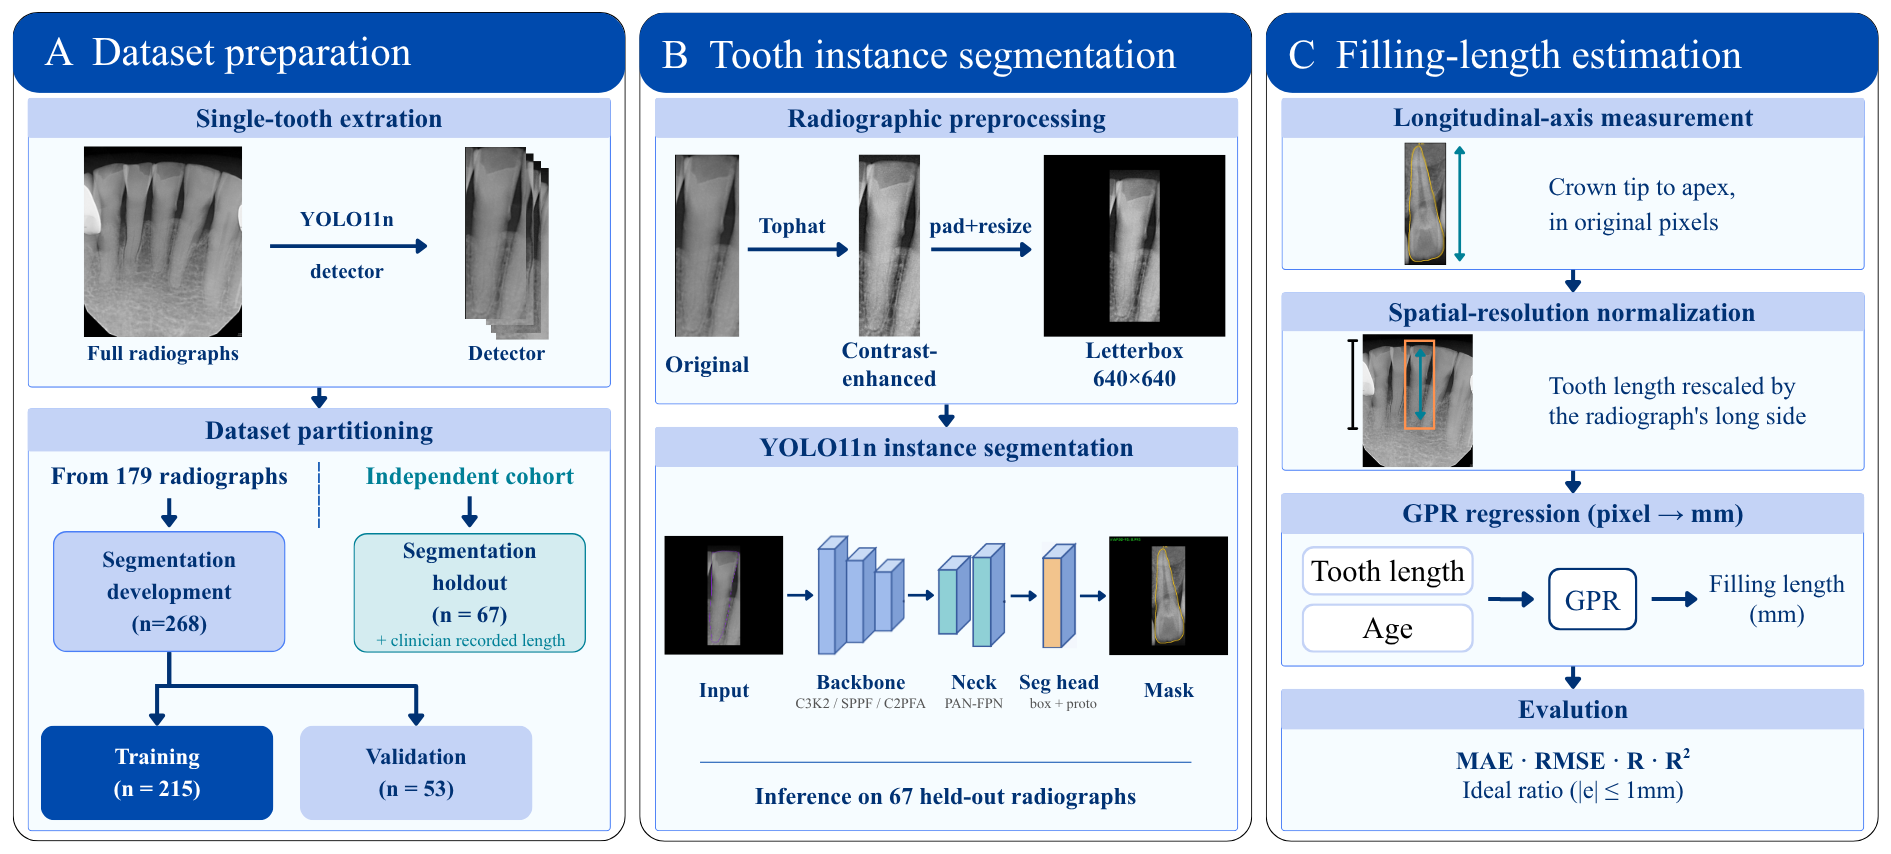
\includegraphics[width=\textwidth]{fig_flowchart.png}
\caption{Overall workflow of the proposed pipeline. (A) Single-tooth extraction and dataset partitioning; (B) top-hat preprocessing and YOLO11n-seg segmentation; (C) longitudinal-axis measurement, long-side normalisation, and GPR-based length conversion.}
\label{fig:workflow}
\end{figure*}

\subsection{Dataset Preparation}

The data were retrospectively collected from patients who had completed root
canal treatment at the Department of Dentistry, Chang Gung Memorial Hospital,
Linkou, Taiwan. All images were de-identified preoperative periapical
radiographs. The study protocol was approved by \tbd{IRB} (approval
no.~\tbd{}). Tooth contours were annotated as polygons (single class
\textit{tooth}) in Roboflow, and the reference filling length was the
post-treatment filling length recorded by the clinicians (mm, resolution
0.25~mm), together with the FDI tooth number, age, and sex.

\paragraph{A. Single-tooth extraction}
Full periapical radiographs usually contain several teeth, alveolar bone, and
surrounding structures. To restrict the subsequent segmentation to the target
tooth, a YOLO11n detector first localises each tooth in the full radiograph and
outputs a two-dimensional bounding box, which is used to crop a single-tooth
image (Figure~\ref{fig:workflow}A). The detector was trained on tooth bounding-box
annotations of 179 full radiographs (training settings in Section~4.1). The 268 images of the segmentation dataset were selected
from the crops of these 179 radiographs, and each of the 67 images of the
length-evaluation dataset was cropped by the same detector into single-tooth
images, from which the target tooth was manually selected according to the
clinician-recorded tooth number.

\paragraph{B. Dataset partitioning}
To avoid information leakage, the 67 images of the length-evaluation dataset were
obtained from patients different from those of the 179 radiographs and served as
an independent test set; only these 67 images have clinician-recorded filling
lengths. The 268 images of the segmentation dataset were randomly split 8:2 into
a training set (215 images) and a validation set (53 images) with a fixed seed of
42 for segmentation-model development. The length-evaluation dataset was never
used for training, validation, or hyperparameter selection of the segmentation
model; it was used only for independent segmentation testing and for
cross-validation of the pixel-to-millimetre conversion, which in turn did not use
the 268 segmentation images. The characteristics of the length-evaluation dataset are summarised in Table~\ref{tab:dataset}.

\begin{table*}[t]
\centering
\caption{Characteristics of the length-evaluation dataset ($n=67$).}
\label{tab:dataset}
\begin{tabular}{@{}llccc@{}}
\toprule
Characteristic & Category & Female & Male & Total \\
 & & ($n=40$) & ($n=27$) & ($n=67$) \\
\midrule
\multirow{4}{*}{Tooth (FDI)} & Maxillary central incisor (11, 21) & 22 & 13 & 35 \\
 & Maxillary lateral incisor (12, 22) & 10 & 8 & 18 \\
 & Mandibular central incisor (31, 41) & 5 & 6 & 11 \\
 & Mandibular lateral incisor (32, 42) & 3 & 0 & 3 \\
\midrule
\multirow{8}{*}{Age (years)} & Mean $\pm$ SD & 39.2 $\pm$ 15.1 & 44.6 $\pm$ 18.7 & 41.4 $\pm$ 16.8 \\
 & 10--19 & 5 & 4 & 9 \\
 & 20--29 & 4 & 4 & 8 \\
 & 30--39 & 9 & 1 & 10 \\
 & 40--49 & 15 & 6 & 21 \\
 & 50--59 & 3 & 5 & 8 \\
 & 60--69 & 2 & 5 & 7 \\
 & 70--79 & 2 & 2 & 4 \\
\midrule
\multirow{6}{*}{\shortstack[l]{Filling length\\(mm)}} & Mean $\pm$ SD & 20.83 $\pm$ 1.68 & 21.22 $\pm$ 1.96 & 20.99 $\pm$ 1.79 \\
 & 17--19 & 4 & 1 & 5 \\
 & 19--21 & 14 & 13 & 27 \\
 & 21--23 & 18 & 6 & 24 \\
 & 23--25 & 3 & 4 & 7 \\
 & 25--27 & 1 & 3 & 4 \\
\bottomrule
\end{tabular}
\end{table*}

\subsection{Tooth Instance Segmentation}

As shown in Figure~\ref{fig:workflow}B, this stage comprises two steps:
radiographic preprocessing (top-hat contrast enhancement followed by padding and
letterboxing) and YOLO11n instance segmentation. It uses the 268 images of the segmentation dataset (215 training,
53 validation) for model development and the 67 images of the length-evaluation
dataset for inference only. All 335 images were preprocessed with identical
parameters.

\paragraph{A. Radiographic preprocessing}
Each single-tooth image $I$ was first contrast-enhanced by a morphological
top-hat transformation,
\begin{equation}
\begin{aligned}
I_{\text{out}} &= I + \mathrm{TH}(I) - \mathrm{BH}(I),\\
\mathrm{TH}(I) &= I - (I \circ B),\\
\mathrm{BH}(I) &= (I \bullet B) - I,
\end{aligned}
\label{eq:tophat}
\end{equation}
where $\circ$ and $\bullet$ denote morphological opening and closing, and $B$ is
a $61\times61$ elliptical structuring element. The white top-hat $\mathrm{TH}$
retains bright structures smaller than $B$, whereas the black top-hat
$\mathrm{BH}$ extracts dark structures smaller than $B$; adding the former and
subtracting the latter accentuates local contrast at the root, root canal, and
alveolar-bone boundaries while suppressing large-scale exposure non-uniformity.
The operation was applied only within the content region (grey level $>10$),
leaving the black border unchanged. For comparison, CLAHE (clip limit 1.5,
$8\times8$ tiles) and the unprocessed images were evaluated with the same
pipeline. Tooth contours were annotated on the CLAHE images; because every
variant alters only pixel intensities and not geometry, the same polygon
annotations were reused for all groups, so that preprocessing was the only
difference between them.

The enhanced image was then padded at the top and bottom by 10\% of its height with
zero-valued pixels and letterboxed to $640\times640$ with its aspect ratio
preserved, and the polygon annotations were transformed accordingly. Compared
with direct resizing, aspect-ratio-preserving scaling avoids geometric distortion
of the root. The scale factor of each image was recorded to map pixel lengths
back to the original resolution.

\paragraph{B. YOLO11n instance segmentation}
Tooth instance segmentation was performed with the segmentation variant of
Ultralytics YOLO11, initialised from \texttt{yolo11n-seg.pt}. YOLO11 extracts
multi-scale features with a C3k2 backbone, aggregates them through a PAN-FPN
neck, and uses a decoupled head to predict class scores and bounding boxes; its
segmentation variant adds mask-coefficient and prototype branches, enabling
tooth detection and pixel-level segmentation in a single forward pass. A single
class (\textit{tooth}) was used. Inference was performed only on the 67 held-out
images. Let $F_\Theta$ denote the segmentation network with parameters $\Theta$;
for a standardised input $R$ it outputs the confidence and mask of each predicted
instance, $M = F_\Theta(R)$. Predictions with confidence $\ge 0.15$ were retained.
Each mask was filled and opened with a $3\times3$ kernel to cut thin bridges, and
only its largest connected component was kept; the target tooth was selected as
the mask whose bounding box had the highest IoU with the reference box.

\subsection{Filling-Length Estimation}

As shown in Figure~\ref{fig:workflow}C, this stage is applied only to the 67
images of the length-evaluation dataset and consists of longitudinal-axis
measurement, spatial-resolution normalisation, GPR regression from pixels to
millimetres, and evaluation.

\paragraph{A. Longitudinal-axis measurement}
Principal component analysis of the polygon vertices of the selected mask yields
its centroid $\mathbf{c}$ and first principal unit vector $\mathbf{u}$. The
vertices with the minimum and maximum projections onto $\mathbf{u}$ define the
crown tip $A$ and the apex $B$, and the pixel length is
\begin{equation}
\begin{aligned}
L_{\text{px}} &= \lVert \mathbf{p}_B - \mathbf{p}_A \rVert,\\
\mathbf{p}_{A,B} &= \mathbf{c} + \mathbf{u}\,\min/\max_i\,\big[(\mathbf{x}_i-\mathbf{c})\cdot\mathbf{u}\big],
\end{aligned}
\label{eq:lpx}
\end{equation}
which is multiplied by the recorded scale factor to return to the original pixel
space. The crown--apex direction follows the FDI tooth number (maxillary crown
downward, mandibular crown upward); when unavailable, the end whose outer 30\%
segment has the larger mean width is taken as the crown.

\paragraph{B. Spatial-resolution normalisation}
Because the radiographs were exported at different resolutions, the px/mm scale
varies between images (coefficient of variation $\approx0.41$ over the 67
images, but only 0.05--0.10 within the same full-image size). The pixel length is
therefore normalised to an equivalent of a 1200-px long side,
\begin{equation}
L_{\text{norm}} = L_{\text{px}} \times 1200 / S,
\label{eq:lnorm}
\end{equation}
where $S$ is the long-side length of the full radiograph in pixels. This
normalisation uses only the image size and no millimetre reference.

\paragraph{C. GPR regression (pixel to millimetre)}
GPR is a non-parametric Bayesian regression model that assumes
$y = f(\mathbf{x}) + \varepsilon$ with $\varepsilon\sim\mathcal{N}(0,\sigma_n^2)$
and places a Gaussian-process prior on the latent function,
$f(\mathbf{x}) \sim \mathcal{GP}\big(h(\mathbf{x})^{\top}\boldsymbol{\beta},\,k(\mathbf{x},\mathbf{x}')\big)$.
A linear basis $h(\mathbf{x}) = [1,\mathbf{x}^{\top}]^{\top}$ is used as the mean
function, so that the GP models only the residual beyond the linear trend, and
the covariance is the squared-exponential kernel
\begin{equation}
k(\mathbf{x},\mathbf{x}') = \sigma_f^2 \exp\!\left(-\frac{\lVert\mathbf{x}-\mathbf{x}'\rVert^2}{2\sigma_L^2}\right),
\label{eq:se}
\end{equation}
where $\sigma_L$ is the length scale and $\sigma_f$ the signal standard deviation.
The predictive distribution has a closed form, and its posterior mean is used as
the length estimate. Unlike neural networks, GPR requires no random
initialisation and its hyperparameters can be estimated from the marginal
likelihood, which suits small-sample regression. Here the input is
$\mathbf{x} = [L_{\text{norm}}, \text{age}]$ and the target is the
clinician-recorded filling length; a feed-forward neural network (ANN) is used as
a comparison model. Following the clinical principle that a slightly short
filling is safer than an overextended one, the final estimate subtracts a fixed
offset:
\begin{equation}
\hat{y} = f(\mathbf{x}) - 0.5~\text{mm}.
\label{eq:offset}
\end{equation}

\paragraph{D. Evaluation}
The corrected estimates $\hat{y}$ are compared with the clinician-recorded
filling lengths using the MAE, RMSE, Pearson correlation coefficient $R$,
coefficient of determination $R^2$, and the ideal ratio, defined as the
proportion of teeth with $|\hat{y}-y|\le 1.0$~mm. The evaluation protocol and
metric definitions are detailed in Section~4.2.
